% :contentReference[oaicite:0]{index=0}
\documentclass[12pt]{article}
\usepackage[margin=1in]{geometry}
\usepackage{amsmath,amssymb,mathtools}
\usepackage{enumitem}
\usepackage{bm}
\usepackage{hyperref}
\usepackage{fancyhdr}
\usepackage{draftwatermark}
\usepackage{xcolor}
\usepackage{tikz}

%------------- TITLE AND METADATA -------------

\newcommand{\CourseCode}{HE2001 }
\newcommand{\CourseName}{Microeconomics II}
\newcommand{\DocType}{Tutorial 1}

\title{
\CourseCode \CourseName \\[0.3em]
\large \DocType
}
\author{
  Academic Year 2025/2026, Semester 2 \\[0.25em]
  \textit{Quantitative Research Society @NTU}
}
\date{\today}

%----------------------------------------------

%------------- HEADER & FOOTER (for page 2 onward) -------------
\fancypagestyle{main}{
  \fancyhf{}
  \fancyhead[L]{\CourseCode \CourseName}
  \fancyhead[R]{\href{https://qrsntu.org}{QRS@NTU}}
  \fancyfoot[C]{\thepage}
  \renewcommand{\headrulewidth}{0.4pt}
  \renewcommand{\footrulewidth}{0pt}
}

%------------- SIMPLE FOOTER (page 1 only) -------------
\fancypagestyle{plainfirst}{
  \fancyhf{}
  \renewcommand{\headrulewidth}{0pt}
  \renewcommand{\footrulewidth}{0pt}
  \fancyfoot[C]{\scriptsize\textcolor{gray}{\textit{For academic reference only. This document is provided for educational purposes and does not constitute an official question paper, answer key, or any formally authorised academic material. Its content is not guaranteed to be complete or accurate.}}}
}

%------------- WATERMARK -------------
\SetWatermarkText{Unofficial — QRS@NTU — qrsntu.org}
\SetWatermarkScale{1}
\SetWatermarkLightness{0.99}
%------------------------------------

\begin{document}

%------------- COVER PAGE -------------
\maketitle
\thispagestyle{plainfirst}
\pagestyle{main}
\bigskip

%====================================================
% OVERVIEW
%====================================================
\begin{center}
  \rule{0.8\textwidth}{0.4pt}\\[4pt]
  \textbf{Overview}\\[2pt]
  \rule{0.8\textwidth}{0.4pt}
\end{center}

\noindent
This tutorial focuses on foundational two-good consumer theory and revealed preference reasoning:
\begin{itemize}[leftmargin=*]
  \item completeness, transitivity, and monotonicity (``increasingness'') of a preference relation;
  \item budget lines, affordability, and geometric interpretation in \(\mathbb{R}^2_+\);
  \item revealed preference comparisons across periods;
  \item why WARP violations cannot be rationalised by increasing preferences;
  \item constructing a (non-increasing / non-monotone) preference that can rationalise observed choices;
  \item limitations of the ``chosen implies preferred'' maxim in applications.
\end{itemize}

\bigskip

%====================================================
% QUESTION 1
%====================================================
\newpage
\section*{Question 1 (Lexicographic-type preference)}
\subsection*{Problem}
Consider the preference relation \(\succeq\) on \(\mathbb{R}^2\) defined by
\[
(x_1,x_2)\succeq (y_1,y_2)
\quad\Longleftrightarrow\quad
\text{either (i) } x_1>y_1,\ \text{or (ii) } x_1=y_1\ \text{and } x_2\ge y_2.
\]
Is this preference relation complete, transitive, and increasing?

\subsection*{Solution}

\subsubsection*{Method 1: Direct verification from definitions}
We recall the standard definitions.

\begin{itemize}[leftmargin=*]
\item \textbf{Completeness:} for all \(x,y\), either \(x\succeq y\) or \(y\succeq x\) (or both).
\item \textbf{Transitivity:} for all \(x,y,z\), if \(x\succeq y\) and \(y\succeq z\), then \(x\succeq z\).
\item \textbf{Increasing (monotone):} if \(x\ge y\) componentwise and \(x\neq y\), then \(x\succ y\) (i.e.\ \(x\succeq y\) and not \(y\succeq x\)).
\end{itemize}

\paragraph{Completeness.}
Fix any \(x=(x_1,x_2)\) and \(y=(y_1,y_2)\). Exactly one of the following holds:
\[
x_1>y_1,\qquad x_1<y_1,\qquad x_1=y_1.
\]
If \(x_1>y_1\), then \(x\succeq y\) by clause (i).
If \(x_1<y_1\), then \(y_1>x_1\), hence \(y\succeq x\) by clause (i).
If \(x_1=y_1\), then either \(x_2\ge y_2\) or \(y_2\ge x_2\); in the first case \(x\succeq y\) by clause (ii), and in the second case \(y\succeq x\) by clause (ii).
Thus \(\succeq\) is complete.

\paragraph{Transitivity.}
Let \(x,y,z\in\mathbb{R}^2\) satisfy \(x\succeq y\) and \(y\succeq z\). We prove \(x\succeq z\) by cases.

\begin{itemize}[leftmargin=*]
\item If \(x_1>y_1\), then necessarily \(y_1\ge z_1\) or \(y_1=z_1\); in either case \(x_1>z_1\), hence \(x\succeq z\) by clause (i).
\item If \(x_1=y_1\) and \(x_2\ge y_2\), then consider \(y\succeq z\):
  \begin{itemize}[leftmargin=*]
  \item If \(y_1>z_1\), then \(x_1=y_1>z_1\), so \(x\succeq z\) by clause (i).
  \item If \(y_1=z_1\) and \(y_2\ge z_2\), then \(x_1=y_1=z_1\) and \(x_2\ge y_2\ge z_2\), so \(x\succeq z\) by clause (ii).
  \end{itemize}
\end{itemize}
In all cases, \(x\succeq z\). Hence \(\succeq\) is transitive.

\paragraph{Increasingness.}
Let \(x\ge y\) componentwise with \(x\neq y\). Then either \(x_1>y_1\) or \(x_1=y_1\) and \(x_2>y_2\).
\begin{itemize}[leftmargin=*]
\item If \(x_1>y_1\), then \(x\succeq y\) by (i). Also \(y\succeq x\) is impossible because it would require \(y_1>x_1\) or \(y_1=x_1\) with \(y_2\ge x_2\), contradicting \(x_1>y_1\). Hence \(x\succ y\).
\item If \(x_1=y_1\) and \(x_2>y_2\), then \(x\succeq y\) by (ii). For \(y\succeq x\) we would need \(y_1>x_1\) (false) or \(y_1=x_1\) and \(y_2\ge x_2\) (false since \(x_2>y_2\)). Hence \(x\succ y\).
\end{itemize}
Therefore \(\succeq\) is increasing.

\[
\boxed{\text{\(\succeq\) is complete, transitive, and increasing.}}
\]

\subsubsection*{Method 2: Identification with lexicographic order}
Define the lexicographic order \(\succeq_{\mathrm{lex}}\) on \(\mathbb{R}^2\) by
\[
x\succeq_{\mathrm{lex}} y
\quad\Longleftrightarrow\quad
\bigl(x_1>y_1\bigr)\ \text{or}\ \bigl(x_1=y_1\ \text{and}\ x_2\ge y_2\bigr).
\]
By inspection, the preference \(\succeq\) is exactly \(\succeq_{\mathrm{lex}}\). We now verify the properties for \(\succeq_{\mathrm{lex}}\).

\paragraph{Completeness.}
For any \(x,y\), if \(x_1\neq y_1\) then the larger first coordinate is lexicographically preferred; if \(x_1=y_1\), then the larger second coordinate is weakly preferred. Hence either \(x\succeq_{\mathrm{lex}} y\) or \(y\succeq_{\mathrm{lex}} x\).

\paragraph{Transitivity.}
Suppose \(x\succeq_{\mathrm{lex}} y\) and \(y\succeq_{\mathrm{lex}} z\).
If \(x_1>y_1\), then \(x_1>z_1\) (since \(y_1\ge z_1\) or \(y_1=z_1\)), so \(x\succeq_{\mathrm{lex}} z\).
If \(x_1=y_1\) and \(x_2\ge y_2\), then either \(y_1>z_1\) (so \(x_1>z_1\)) or \(y_1=z_1\) and \(y_2\ge z_2\) (so \(x_2\ge z_2\) with \(x_1=z_1\)). In both cases \(x\succeq_{\mathrm{lex}} z\).

\paragraph{Increasingness.}
If \(x\ge y\) and \(x\neq y\), then either \(x_1>y_1\) or \(x_1=y_1\) and \(x_2>y_2\); either way \(x\succ_{\mathrm{lex}} y\). Hence increasingness holds.

\[
\boxed{\text{\(\succeq\) is lexicographic-type: complete, transitive, and increasing.}}
\]

%====================================================
% QUESTION 2
%====================================================
\newpage
\section*{Question 2 (Budget lines and affordability)}
\subsection*{Problem}
Draw the budget line for prices \(p^{(1)}=(1,2)\) and \(p^{(2)}=(2,1)\) when expenditure is \(m=2\).
Draw the consumption bundle \(x=(1,1)\).
Is this bundle affordable at either budget?

\subsection*{Solution}

\subsubsection*{Method 1: Geometric check (point lies above each line)}

\begin{figure}[h!]
\centering
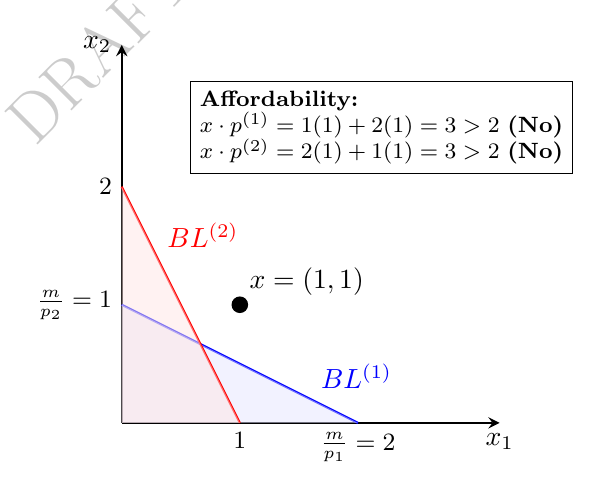
\begin{tikzpicture}[scale=1.5, >=stealth]
  % --- 1. Axes ---
  \draw[->, thick] (0,0) -- (3.2,0) node[below] {$x_1$};
  \draw[->, thick] (0,0) -- (0,3.2) node[left] {$x_2$};

  % --- 2. Budget Line 1: p1*x1 + p2*x2 = m => 1*x1 + 2*x2 = 2 ---
  % Intercepts: (2,0) and (0,1)
  \draw[blue, thick] (0,1) -- (2,0) node[above right, pos=0.8] {$BL^{(1)}$};
  \fill[blue!10, opacity=0.5] (0,0) -- (0,1) -- (2,0) -- cycle;

  % --- 3. Budget Line 2: p1*x1 + p2*x2 = m => 2*x1 + 1*x2 = 2 ---
  % Intercepts: (1,0) and (0,2)
  \draw[red, thick] (0,2) -- (1,0) node[above right, pos=0.3] {$BL^{(2)}$};
  \fill[red!10, opacity=0.5] (0,0) -- (0,2) -- (1,0) -- cycle;

  % --- 4. Consumption Bundle x = (1,1) ---
  \coordinate (X) at (1,1);
  \fill (X) circle (2pt) node[above right] {$x = (1,1)$};

  % --- 5. Labels for Intercepts ---
  % For BL1
  \node[left, font=\small] at (0,1) {$\frac{m}{p_2}=1$};
  \node[below, font=\small] at (2,0) {$\frac{m}{p_1}=2$};
  % For BL2
  \node[left, font=\small] at (0,2) {2};
  \node[below, font=\small] at (1,0) {1};

  % --- 6. Legend/Notes ---
  \node[draw, fill=white, font=\footnotesize, align=left] at (2.2, 2.5) {
    \textbf{Affordability:}\\
    $x \cdot p^{(1)} = 1(1) + 2(1) = 3 > 2$ \textbf{(No)}\\
    $x \cdot p^{(2)} = 2(1) + 1(1) = 3 > 2$ \textbf{(No)}
  };

\end{tikzpicture}
\caption{Budget sets for $p^{(1)}=(1,2)$ and $p^{(2)}=(2,1)$ with $m=2$. The bundle $x=(1,1)$ lies outside both budget sets.}
\end{figure}

For \(p^{(1)}\), feasibility on/under the line requires \(x_1+2x_2\le 2\). At \((1,1)\),
\[
1+2(1)=3>2,
\]
so \((1,1)\) lies above that line.

For \(p^{(2)}\), feasibility on/under the line requires \(2x_1+x_2\le 2\). At \((1,1)\),
\[
2(1)+1=3>2,
\]
so \((1,1)\) lies above that line too.

\[
\boxed{\text{Graphically, \(x=(1,1)\) lies above both budget lines, hence is infeasible.}}
\]

\subsubsection*{Method 2: Write the budget line equations and evaluate costs}



For a two-good economy, the budget line with prices \(p=(p_1,p_2)\) and expenditure \(m\) is
\[
p_1 x_1 + p_2 x_2 = m.
\]

\paragraph{Budget line for \(p^{(1)}=(1,2)\), \(m=2\).}
The equation is
\[
x_1 + 2x_2 = 2.
\]
Intercepts: \((2,0)\) and \((0,1)\).

\paragraph{Budget line for \(p^{(2)}=(2,1)\), \(m=2\).}
The equation is
\[
2x_1 + x_2 = 2.
\]
Intercepts: \((1,0)\) and \((0,2)\).

\paragraph{Affordability of \(x=(1,1)\).}
Compute expenditures:
\[
p^{(1)}\cdot x = 1\cdot 1 + 2\cdot 1 = 3,\qquad
p^{(2)}\cdot x = 2\cdot 1 + 1\cdot 1 = 3.
\]
Since \(3>2\), the bundle is not affordable under either budget.

\[
\boxed{\text{\(x=(1,1)\) is not affordable under either budget.}}
\]



%====================================================
% QUESTION 3
%====================================================
\newpage
\section*{Question 3 (Revealed preference across periods)}
\subsection*{Problem}
Suppose a preference-maximising consumer in period 1 buys \(x^{1}=(2,2)\) when prices are \(p^{1}=(1,1)\),
and buys \(x^{2}=(0,3)\) in period 2 when prices are \(p^{2}=(2,1)\).
In which period is the consumer better off (i.e.\ in which period does the consumer obtain a better bundle)?

\subsection*{Solution}

\subsubsection*{Method 1: Direct revealed-preference comparison via affordability}
Let \(m^t:=p^t\cdot x^t\) be the expenditure in period \(t\). Compute:
\[
m^1 = p^1\cdot x^1 = 1\cdot 2 + 1\cdot 2 = 4,\qquad
m^2 = p^2\cdot x^2 = 2\cdot 0 + 1\cdot 3 = 3.
\]
Check whether \(x^2\) was affordable in period 1:
\[
p^1\cdot x^2 = 1\cdot 0 + 1\cdot 3 = 3 \le 4,
\]
so \(x^2\) was feasible when \(x^1\) was chosen. Therefore, period-1 optimality implies
\[
x^1 \succeq x^2.
\]
Check the reverse affordability in period 2:
\[
p^2\cdot x^1 = 2\cdot 2 + 1\cdot 2 = 6 > 3,
\]
so \(x^1\) was not feasible in period 2; hence period 2 cannot reveal \(x^2\succeq x^1\).

\[
\boxed{\text{The consumer is (weakly) better off in period 1: } x^{1}\succeq x^{2}.}
\]

\subsubsection*{Method 2: Cross-expenditure inequalities (``price-index'' view)}
From period 1, choosing \(x^1\) at \(p^1\) means every bundle with weakly lower period-1 cost cannot be strictly preferred to \(x^1\):
\[
p^1\cdot x \le p^1\cdot x^1 \ \Longrightarrow\ x^1\succeq x.
\]
Since
\[
p^1\cdot x^2 = 3 \le 4 = p^1\cdot x^1,
\]
we conclude \(x^1\succeq x^2\).

Meanwhile,
\[
p^2\cdot x^1 = 6 > 3 = p^2\cdot x^2,
\]
so period 2 provides no basis to infer \(x^2\succeq x^1\).

\[
\boxed{x^1 \succeq x^2\ \text{is the only welfare conclusion supported by the data.}}
\]

%====================================================
% QUESTION 4
%====================================================
\newpage
\section*{Question 4 (WARP violation and impossibility under increasing preferences)}
\subsection*{Problem}
Consider a consumer who buys \(x^{1}=(1,2)\) when prices are \(p^{1}=(1,2)\) and buys \(x^{2}=(2,1)\) when prices are \(p^{2}=(2,1)\).
The consumer does not satisfy WARP.
Prove that there is no increasing preference \(\succeq\) which can explain the consumer's behaviour.
That is, show that there is no increasing \(\succeq\) such that
\[
x^{1}\succeq x \ \text{for all } x\in B(p^{1},\,p^{1}\cdot x^{1}),
\qquad
x^{2}\succeq x \ \text{for all } x\in B(p^{2},\,p^{2}\cdot x^{2}).
\]

\subsection*{Solution}

\subsubsection*{Method 1: Contradiction via strict improvement from ``slack''}
Compute the expenditures:
\[
m^1=p^{1}\cdot x^{1} = 1\cdot 1 + 2\cdot 2 = 5,
\qquad
m^2=p^{2}\cdot x^{2} = 2\cdot 2 + 1\cdot 1 = 5.
\]

\paragraph{Step 1: Mutual affordability forces mutual weak preference.}
Cross-affordability:
\[
p^{1}\cdot x^{2} = 1\cdot 2 + 2\cdot 1 = 4 \le 5
\quad\Rightarrow\quad
x^{1}\succeq x^{2},
\]
\[
p^{2}\cdot x^{1} = 2\cdot 1 + 1\cdot 2 = 4 \le 5
\quad\Rightarrow\quad
x^{2}\succeq x^{1}.
\]
So any rationalising \(\succeq\) would imply \(x^1\sim x^2\).

\paragraph{Step 2: Increasingness yields a feasible bundle strictly better than \(x^2\) in period 1.}
Because \(p^{1}\cdot x^{2}=4<5\), the bundle \(x^{2}\) leaves strictly positive expenditure unused under \(p^1\).
Use the remaining \(1\) unit of expenditure to increase good 1 (priced at \(1\) under \(p^1\)):
\[
y := x^{2} + (1,0) = (3,1).
\]
Then
\[
p^{1}\cdot y = p^{1}\cdot x^{2} + p^{1}\cdot(1,0)=4+1=5,
\]
so \(y\in B(p^{1},m^1)\). Also \(y\ge x^2\) and \(y\neq x^2\), hence by increasingness \(y\succ x^2\).

\paragraph{Step 3: Period-1 optimality forces \(x^1\succ x^2\), contradicting period-2 optimality.}
Since \(y\in B(p^1,m^1)\) and \(x^1\) is optimal there, \(x^1\succeq y\). With \(y\succ x^2\) and transitivity, \(x^1\succ x^2\).
But \(x^1\succ x^2\) means \emph{not} \(x^2\succeq x^1\), contradicting the earlier implication \(x^2\succeq x^1\).

\[
\boxed{\text{No increasing preference \(\succeq\) can rationalise these two choices.}}
\]

\subsubsection*{Method 2: General lemma --- increasing preferences imply WARP}
\paragraph{Lemma.}
Assume \(\succeq\) is increasing and choices \(x^1,x^2\) are \(\succeq\)-maximisers on their respective budget sets.
Then it is impossible to have both \(p^1\cdot x^2\le p^1\cdot x^1\) and \(p^2\cdot x^1\le p^2\cdot x^2\) with at least one inequality strict and \(x^1\neq x^2\).
(That is, increasing rationalisable data must satisfy WARP.)

\paragraph{Proof.}
Assume for contradiction that \(x^2\) is affordable when \(x^1\) is chosen and \(x^1\) is affordable when \(x^2\) is chosen, with (say) \(p^1\cdot x^2 < p^1\cdot x^1\).
Then optimality gives \(x^1\succeq x^2\) and \(x^2\succeq x^1\), so \(x^1\sim x^2\).

Let \(\Delta := p^1\cdot x^1 - p^1\cdot x^2>0\).
Because prices are positive, pick \(i\in\{1,2\}\) and \(\varepsilon>0\) such that \(p^1_i\varepsilon\le \Delta\).
Set \(y:=x^2+\varepsilon e_i\). Then \(y\ge x^2\), \(y\neq x^2\), and
\[
p^1\cdot y = p^1\cdot x^2 + p^1_i\varepsilon \le p^1\cdot x^2 + \Delta = p^1\cdot x^1,
\]
so \(y\) is feasible in period 1. Increasingness gives \(y\succ x^2\), and period-1 optimality gives \(x^1\succeq y\), hence \(x^1\succ x^2\), contradicting \(x^2\succeq x^1\).

\paragraph{Apply to the data.}
Here \(p^1\cdot x^2=4<5=p^1\cdot x^1\) and \(p^2\cdot x^1=4<5=p^2\cdot x^2\), so the lemma gives a contradiction immediately.

\[
\boxed{\text{Since the choices violate WARP, no increasing rationalising preference exists.}}
\]

%====================================================
% QUESTION 5
%====================================================
\newpage
\section*{Question 5 (Constructing a non-increasing preference that rationalises the choices)}
\subsection*{Problem}
Define a non-increasing preference \(\succeq\) which can explain the behaviour of the consumer in the previous question.

\subsection*{Solution}

\subsubsection*{Method 1: Norm-minimising (``smaller bundles are better'') preference}
Define \(\succeq\) on \(\mathbb{R}^2_+\) by
\[
x\succeq y \quad\Longleftrightarrow\quad \|x\|_2 \le \|y\|_2,
\]
equivalently via the utility \(u(x):=-\|x\|_2^2=-(x_1^2+x_2^2)\).

\paragraph{Non-increasingness.}
If \(x\ge y\) componentwise, then \(x_1^2\ge y_1^2\) and \(x_2^2\ge y_2^2\), hence
\[
\|x\|_2^2 \ge \|y\|_2^2 \quad\Rightarrow\quad y\succeq x.
\]
So ``more of both goods'' cannot improve welfare; the preference is non-increasing.

\paragraph{Rationalisation on the budget lines of Question 4.}
In Question 4, \(m^1=m^2=5\) and the budget lines are
\[
x_1+2x_2=5,\qquad 2x_1+x_2=5.
\]
Under \(u(x)=-\|x\|_2^2\), the consumer chooses the bundle on each line that \emph{minimises} \(\|x\|_2^2\).

\paragraph{Period 1.}
Minimise \(x_1^2+x_2^2\) subject to \(x_1+2x_2=5\).
Lagrangian \(\mathcal{L}=x_1^2+x_2^2+\lambda(x_1+2x_2-5)\).
FOCs:
\[
2x_1+\lambda=0,\qquad 2x_2+2\lambda=0.
\]
So \(\lambda=-2x_1\) and \(2x_2-4x_1=0\Rightarrow x_2=2x_1\).
Impose the constraint: \(x_1+2(2x_1)=5\Rightarrow 5x_1=5\Rightarrow x_1=1\), hence \(x_2=2\).
Thus \(x^1=(1,2)\) is optimal on the first budget line.

\paragraph{Period 2.}
Minimise \(x_1^2+x_2^2\) subject to \(2x_1+x_2=5\).
Lagrangian \(\mathcal{L}=x_1^2+x_2^2+\lambda(2x_1+x_2-5)\).
FOCs:
\[
2x_1+2\lambda=0,\qquad 2x_2+\lambda=0.
\]
Thus \(\lambda=-x_1=-2x_2\Rightarrow x_1=2x_2\).
Impose the constraint: \(2(2x_2)+x_2=5\Rightarrow 5x_2=5\Rightarrow x_2=1\), hence \(x_1=2\).
Thus \(x^2=(2,1)\) is optimal on the second budget line.

\[
\boxed{\text{One rationalising non-increasing preference is } u(x)=-(x_1^2+x_2^2).}
\]

\subsubsection*{Method 2: Cauchy--Schwarz (closed-form optimiser on a budget line)}
For any \(p\in\mathbb{R}^2_{++}\) and \(m>0\), consider the budget line \(p\cdot x=m\).
By Cauchy--Schwarz,
\[
(p\cdot x)^2 \le \|p\|_2^2\,\|x\|_2^2.
\]
If \(p\cdot x=m\), then
\[
\|x\|_2^2 \ge \frac{m^2}{\|p\|_2^2},
\]
with equality if and only if \(x\) is a nonnegative scalar multiple of \(p\), i.e.\ \(x=\alpha p\).
Imposing \(p\cdot x=m\) yields \(\alpha=m/\|p\|_2^2\), hence the unique norm-minimiser is
\[
x^\star=\frac{m}{\|p\|_2^2}\,p.
\]

Apply with \(m=5\).

\paragraph{Period 1.} \(p^1=(1,2)\), \(\|p^1\|_2^2=1^2+2^2=5\), so
\[
x^\star=\frac{5}{5}(1,2)=(1,2)=x^1.
\]

\paragraph{Period 2.} \(p^2=(2,1)\), \(\|p^2\|_2^2=2^2+1^2=5\), so
\[
x^\star=\frac{5}{5}(2,1)=(2,1)=x^2.
\]

\[
\boxed{x^t=\frac{m^t}{\|p^t\|_2^2}\,p^t\ \text{under } u(x)=-\|x\|_2^2,\ \ t=1,2.}
\]

%====================================================
% QUESTION 6
%====================================================
\newpage
\section*{Question 6 (When ``chosen implies preferred'' can be problematic)}
\subsection*{Problem}
The first maxim of classic consumer theory states that
\emph{``What is chosen is preferred to what could have been chosen.''}
Can you think of some situations where this maxim may be problematic?

\subsection*{Solution}

\subsubsection*{Method 1: The analyst's ``could have been chosen'' set may be wrong}
The maxim assumes the analyst correctly observes the decision maker's true feasible set.
In practice, a budget constraint used by the analyst may omit real constraints faced by the consumer.

Examples:
\begin{itemize}[leftmargin=*]
\item \textbf{Availability constraints:} stockouts, rationing, or per-customer limits mean some ``affordable'' bundles were not actually feasible.
\item \textbf{Transaction/search costs:} time, transportation, fees, or information frictions reduce the effective opportunity set.
\item \textbf{Indivisibilities:} if goods come in integer units, many points on a continuous budget line cannot be chosen.
\item \textbf{Institutional constraints:} eligibility rules, contracts, penalties, or required bundles restrict feasible options.
\end{itemize}

\subsubsection*{Method 2: Observed choice may not reveal stable preference maximisation}
Even if feasibility is correctly measured, observed choice can be contaminated by factors outside a stable preference-maximisation model.

Examples:
\begin{itemize}[leftmargin=*]
\item \textbf{Mistakes/limited attention:} the consumer may choose a dominated option due to errors or cognitive constraints.
\item \textbf{Uncertainty/incomplete information:} ex ante choice may not align with ex post preference comparisons.
\item \textbf{Time inconsistency:} short-run and long-run selves may disagree, so choice may not reflect the welfare-relevant preference.
\item \textbf{Social/strategic motives:} signalling, norms, or incentives can drive choice in ways not captured by the model.
\end{itemize}


\end{document}
